 %!TEX program = pdflatex
\documentclass[11pt]{article}
\usepackage{amsmath,textcomp,amssymb,graphicx,cancel}
\usepackage{gensymb}
\usepackage[margin=1in]{geometry}
\usepackage{pgfplots}
\pgfplotsset{width=7cm,compat=1.8}
%\usepackage{fontspec}
% \setmainfont
%   []
%   {SourceCodePro-Regular.otf}

\usepackage[colorlinks, urlcolor=blue]{hyperref}
\usepackage{tikz}
\usepackage{epigraph}
%\setlength\parindent{24pt}

\def\Name{Zackery Field}  % Your name
\def\Session{Fall 2013} %Semester

\title{BIOE147 -- Fall 2013 -- PS1}
\author{\Name}
\markboth{BIOE147 \Session \Name}{\Name -- PS1}
\pagestyle{myheadings}

\renewcommand\epigraphflush{flushright}
\renewcommand\epigraphsize{\normalsize}
\setlength\epigraphwidth{0.7\textwidth}

\definecolor{titlepagecolor}{cmyk}{1,.60,0,.40}

% The following code is borrowed from: http://tex.stackexchange.com/a/86310/10898

\newcommand\titlepagedecoration{%
\begin{tikzpicture}[remember picture,overlay,shorten >= -10pt]

\coordinate (aux1) at ([yshift=-15pt]current page.north east);
\coordinate (aux2) at ([yshift=-410pt]current page.north east);
\coordinate (aux3) at ([xshift=-4.5cm]current page.north east);
\coordinate (aux4) at ([yshift=-150pt]current page.north east);

\begin{scope}[titlepagecolor!40,line width=12pt,rounded corners=12pt]
\draw
  (aux1) -- coordinate (a)
  ++(225:5) --
  ++(-45:5.1) coordinate (b);
\draw[shorten <= -10pt]
  (aux3) --
  (a) --
  (aux1);
\draw[opacity=0.6,titlepagecolor,shorten <= -10pt]
  (b) --
  ++(225:2.2) --
  ++(-45:2.2);
\end{scope}
\draw[titlepagecolor,line width=8pt,rounded corners=8pt,shorten <= -10pt]
  (aux4) --
  ++(225:0.8) --
  ++(-45:0.8);
\begin{scope}[titlepagecolor!70,line width=6pt,rounded corners=8pt]
\draw[shorten <= -10pt]
  (aux2) --
  ++(225:3) coordinate[pos=0.45] (c) --
  ++(-45:3.1);
\draw
  (aux2) --
  (c) --
  ++(135:2.0) --
  ++(45:2.0) --
  ++(-45:2.5) coordinate[pos=0.3] (d);   
\draw 
  (d) -- +(45:1);
\end{scope}
\end{tikzpicture}
}

\begin{document}
% \sffamily
% \fontspec
%   []
%   {SourceCodePro-Regular.otf}
\maketitle
%\titlepagedecoration
\section*{1. Genetic Logic}

{\centering
  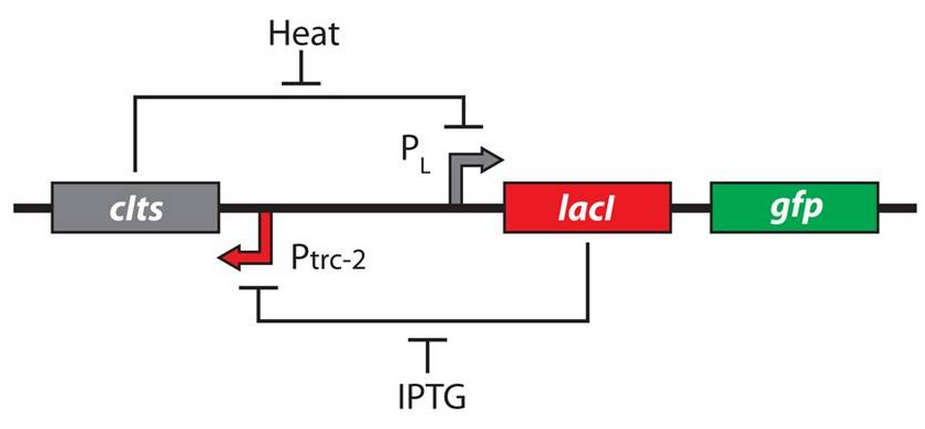
\includegraphics[scale=0.3, trim = 0mm 0mm 7mm 0mm, clip]{ps1_q1.png}\par
  Khalil, Collins 2010\par
}
\begin{itemize}

\item[(a.)]For all input combinations of the above circuit, complete and explain the truth table for steady state outputs.

{
  \centering
  \begin{tabular}{ c | c || c }
  Heat & IPTG  & GFP \\
  \hline
  1 & 1 & 1 \\
  1 & 0 & 1 \\
  0 & 1 & 0 \\
  0 & 0 & state memory \\
  \end{tabular}
  \par
}

The presence of both heat and IPTG lead the deactiviation of both repression signals and therefore the constitutive promotion of all three protein coding sequences: clts, IPTG, and GFP. The presence of heat alone will deactivate clts repression of the $P_L$ promoter and therefore lead to transcription of GFP and lacI. In the heat only case, the production of lacI also downregulates the transcription of clts. The presence of IPTG alone will deactivate the repression of the $P_{trc-2}$ promoter, which leads to the repression of the $P_L$ promoter and the downregulation of GFP transcription. In the final case, no IPTG or heat, the system will remain in whichever state it was found before. There is a subtly to this last case which involves production of clts in the heat-only case. In the heat-only case there was no clts being produced (and whatever was previously there is denatured), so the removal of heat from the system (the no IPTG, no heat case)  would not lead to the repression of the $P_L$ promoter and transcription of GFP would continue. 

\item[(b.)]If you induce the system with a pulse of IPTG, what would you expect the output to be over time?

As described above, the system was designed to maintain its most recent state after the removal of both IPTG and heat from the system. The case of maintaining the OFF position (GFP not transcribed) relies on the continued repression of the $P_L$ promoter. This repression relies on the clts repressor protein. If the length of time that the IPTG pulse is applied is shorter than the degradation time of lacI, then once the IPTG is removed there will be repression of the $P_{trc-2}$, which will lead to the downregulation of clts production. With both promoters now being repressed, the steady state of the system is dependent upon degradation rates of clts and lacI. This is an unstable state as the initial degradation of either protein will lead to the downregulation of transcription of that same protein. 

\item[(c.)]What useful properties does the circuit have?

It has one bit state memory (GFP:ON/OFF). A common application of systems with one bit state memory is with toggle switches (i.e. car ignitions, light switches).

\item[(d.)]Say you add a pulse of heat to the circuit and see GFP expression peak then gradually decay. Is this the expected output? What is a potential mechanism for this behavior? How could you revise the circuit to sustained GFP expression?

This is not the expected output. As stated in (a.), the state of the system should be maintained after inputs are removed. Assuming that heat denatured all clts repressor proteins, there could be some leaky expression at the $P_{trc-2}$ promoter that could cause the decay of GFP. If the clts protein is expressed even when the $P_{trc-2}$ promoter is bound, then this could lead to the increasing repression of the lacI$\cdot $GFP coding region. The system would then remain in the off state until more heat was added. 

In order to sustain GFP expression in the face of leaky expression of clts, you could introduce a promoter at the $P_{trc-2}$ site that has tighter expression.

\item[(e.)]Say you apply a pulse of heat to the system (GFP is off initially). Draw qualitatively what the GFP fluorescence would look like over time in the case of constant IPTG at different levels.
\newline
\pgfplotsset{ 
    samples=15,
    width=10cm,
    xlabel=time,
    ylabel=GFP,
    yticklabels={},
    xticklabels={},
    }
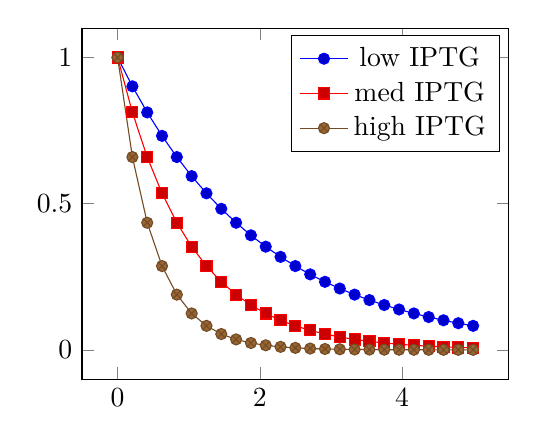
\begin{tikzpicture}
\begin{axis}
% \begin{semilogyaxis}[
%     log plot exponent style/.style={
%         /pgf/number format/fixed zerofill,
%         /pgf/number format/precision=1},
%     domain=-5:10]
  \addplot+[domain=0:5]
    {exp(-x/2)} ;
  \addplot+[domain=0:5] 
    {exp(-x)};
  \addplot+[domain=0:5]
    {exp(-x*2)};
  \legend{low IPTG,med IPTG, high IPTG}
\end{axis}
\end{tikzpicture}

After the pulse of heat in each case there is the same initial GFP concentration. At steady state there each case also has the same GFP concentration ($\sim 0$). So the only difference is the rate at which GFP concentration decreases. This rate is proportional to the concentration of IPTG. Not pictured is the limit at which IPTG concentration no longer effects the rate of GFP decrease because all lacI proteins are bound to IPTG.

\end{itemize}



\section*{2. Modeling}

Say you want to model the circuit described above using the following simplifications: the $P_{L}$-LacI DNA (DNA$_{1}$) can be reversibly bound by λ Cl repressor ($P_{2}$) to form an inactive DNA$_{1}\cdot P_{2}$ complex in a second order reaction. Free DNA$_{1}$ is transcribed in a first order reaction to instantaneously form RNA$_{1}$ (DNA$_{1}$ is not consumed) and RNA$_{1}$ undergoes first order degradation. RNA$_{1}$ is transcribed in a first order reaction to LacI($P_{1}$) and $P_{1}$ undergoes first order degradation. The same process occurs for DNA$_{2}$ which is reversibly inactivated by $P_{1}$ while RNA$_{2}$ and $P_{2}$ undergo first order synthesis and degradation. For the sake of simplicity, assume that protein$\cdot$DNA binding does not significantly alter the concentration of protein. 




{
  \centering
  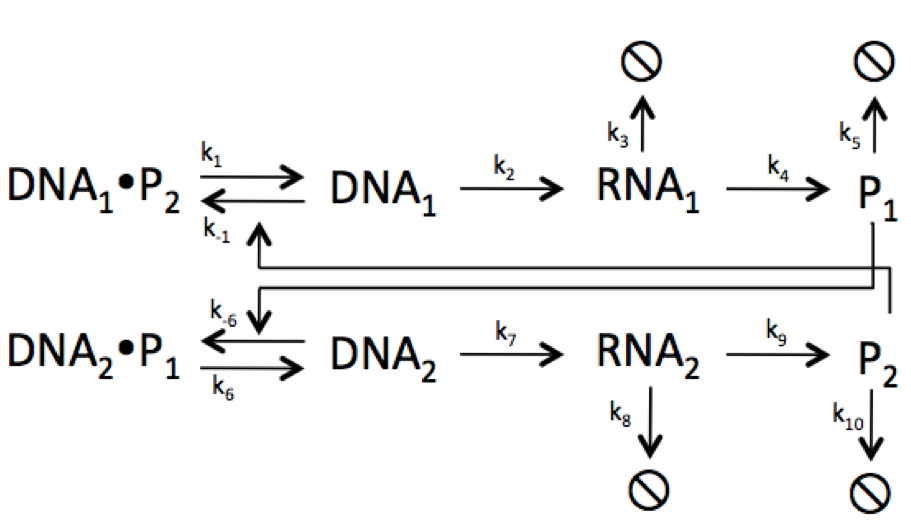
\includegraphics[scale=0.3]{ps1_q2.png} \par
}

\begin{itemize}

\item[(a.)]Write differential equations for all relevant species in the model

\begin{equation*}
  \begin{aligned}
  %Top equations
  \frac{d(\mbox{DNA}_1\cdot P_2)}{dt}&=k_{-1}[P_2][\mbox{DNA}_1] -k_1 [\mbox{DNA}_1\cdot P_2]\\
  \frac{d(\mbox{DNA}_1)}{dt}&=k_1[\mbox{DNA}_1\cdot P_2]-k_{-1}[\mbox{DNA}_1][P_2]\\
  \frac{d(\mbox{RNA}_1)}{dt}&=k_2[\mbox{DNA}_1]-k_3[\mbox{RNA}_1]\cancel{-k_4[\mbox{RNA}_1]}\\
  \frac{d(P_1)}{dt}&=k_4[\mbox{RNA}_1]-k_5[P_1] \cancel{-k_{-6}[\mbox{DNA}_2][P_1]}\\
  %Bottom equations
  \frac{d(\mbox{DNA}_2\cdot P_1)}{dt}&=k_{-6}[P_1][\mbox{DNA}_2] -k_6 [\mbox{DNA}_1\cdot P_1]\\
  \frac{d(\mbox{DNA}_2)}{dt}&=k_6[\mbox{DNA}_2\cdot P_1]-k_{-6}[\mbox{DNA}_2][P_1]\\
  \frac{d(\mbox{RNA}_2)}{dt}&=k_7[\mbox{DNA}_2]-k_8[\mbox{RNA}_2]\cancel{-k_9[\mbox{RNA}_2]}\\
  \frac{d(P_2)}{dt}&=k_9[\mbox{RNA}_2]-k_{10}[P_2] \cancel{-k_{-1}[\mbox{DNA}_1][P_2]}
  \end{aligned}
\end{equation*}


\item[(b.)]Find an expression for the steady state level of DNA$_{1}$
 (and thus $P_{1}$) in terms of the relevant constants. You can assume rate constants for RNA and proteins are similar between LacI and cl-ts clusters. What does the steady state level of DNA$_{1}$approach as you add a large number of repeats of DNA$_{2}$? What if you add many repeats of DNA$_{1}$ instead? 

Assumptions:
\begin{itemize}
\item RNA is not depleted when it is translates into $P$, or RNA depletion is dominated by its first-order degradation.
\item The amount of DNA$_{1,2}$ is constant $[\mbox{DNA}_i]+[\mbox{DNA}_i\cdot P_{(-i\mod3)}]=[\mbox{DNA}_i]_0$
\item The repressor proteins are in instantaneous equilibrium with their respective DNA segements. $$k_f[\mbox{DNA}\cdot P]=k_r[\mbox{DNA}][P]$$
\item The amount of free/bound DNA is at equilibrium at the time-scale of $P_1$ formation. $$k_f[\mbox{DNA}\cdot P]=k_r[\mbox{DNA}][P] + k_{cat}[\mbox{DNA}\cdot P] $$
where $k_{cat}$ encompasses transcription and translation.
\end{itemize}
Here is the general form of this type of interaction with transcraption and translation abstracted away. What has been abstracted does not alter the general behavior of the system, but when designing the actual system taking into account the degradation of RNA, and the speed at which the system can respond (from repression downregulation to protein production) would be important.
\begin{equation*}
  \begin{aligned}
  {[\mbox{DNA}]} = \frac{[\mbox{DNA}]_0}{K_m[P]+1},K_m=\frac{k_r+k_{cat}}{k_f}
  \end{aligned}
\end{equation*}

And here are the coupled interactions of $\mbox{DNA}_1$ with $P_2$ as well as DNA$_2$ with $P_1$, and also the velocities of protein production. $V_{max}=k_{cat}[\mbox{DNA}_i]_0$

\begin{equation}
  \begin{aligned}
    {[\mbox{DNA}_1]} &= \frac{[\mbox{DNA}_1]_0}{K_{m1}[P_2]+1}\\
    {[\mbox{DNA}_2]} &= \frac{[\mbox{DNA}_2]_0}{K_{m2}[P_1]+1}\\
    v_1=\frac{d[P_1]}{dt}&= k_{cat1}[\mbox{DNA}_1] = \frac{V_{max1}}{K_{m1}[P_2]+1}\\
    v_2=\frac{d[P_2]}{dt}&= k_{cat2}[\mbox{DNA}_2] = \frac{V_{max2}}{K_{m2}[P_1]+1}
  \end{aligned}
\end{equation}

Once again, we are ignoring the first order degradation for simplicity. It does affect the rate of production, but only by some constant factor. We can see from equation $(1)$ that the steady-state level of $[\text{DNA}_1]$ is inversely proportional to concentration of $P_2$. $V_{max2}$ would increase with the increased repeats of $[\text{DNA}_2]$, and this would result in increased $P_2$ production (see eq. $(4)$). Looking back to eq. $(1)$, this increased $[P_2]$ would result in a decrease in $[\text{DNA}_1]$. The inverse relationship also holds for increased $[\text{DNA}_1]$ repeats.  
\item[(c.)]Is this model relevant for circuits that have been integrated into the genome? What about circuits on plasmids transformed into E. coli

One of the major assumptions of Michaelis Menten kinetics that is not mentioned above is the reliance upon free diffusion of the species. This is not at all the case in the cell, especially with only a single DNA molecule, and also when you consider then density of the interior of the cell.  If this circuit is on the genome then it is much more difficult to regulate transcription, and this is due to the complexity of available sigma factors among many other things. Another assumption of this model is that the repressor proteins and their DNA segments associate/dissociate quickly enough that they are always in equilibrium. This won't be the case if the site of protein production is far from the particular DNA segment that it binds to. There is hope that this model will be applicable to this circuit if it is located on a plasmid and transformed into E. coli, but it would depend on the particular implementation of the circuit and its ability to overcome the faults in the model (noise, diffusion, etc). 
\end{itemize}


\section*{3. Circuit Design and DNA Assembly}

Use dox, IPTG, ATG, as small molecule signals, and then also siRNA

One to one signal to response. In the 3-way toggle form

\begin{itemize}
\item[(a.)] If you want to extend the circuit to include three states in mammalian cells how would you design the new circuit given the parts below. 

{
  % \centering
  \hspace*{-3cm}\includegraphics[scale=.7, trim = 0mm 0mm 7mm 0mm, clip]{"3-way_toggle_vector"}\par
}

Note: IPTG can be used to cancel LacO1 repression. dox can be used to cancel TetR repression. Inserting cRNA (or cDNA) for the FF4shRNA sequence could be used to cancel repression of the FF4 target in the 3' intron by competitively binding to the FF4shRNA. 
\item[(b.)] What do you predict the main challenges will be in implementing the circuit you designed?

I am not at all familiar with shRNA mechanism and I presume that I would run into some trouble there. The biggest obstacle I see with this is cleaving of the 3' UTR after BFP. If that region is cleaved then the FF4 shRNA transcribed by the other two "switches" will have no effect in reducing the output of BFP. 

There are also quite a few fine tuning aspects that would have to be considered including: the repressibility of each switch, the degradation of FF4 shRNA, and the promoter strength of each switch.
\item[(c.)] How does the total number of circuit elements needed for your circuit scale with the number of states desired?

The possible complexity of a circuit is related exponentially to the number of elements in it (at least theoretically). 

\item[(d.)] Describe how you would assemble your circuit given that you have access to BioBricks and Gateway entry vectors for all promoter/operator combinations and for all genes, and also any primers you may need up to 60bp. You can also design your BioBrick backbones or Gateway destination vectors if that speeds up your assembly. Note: Assume that the cell line you are studying is hard to transfect. 

Since there are so many parts that need to be cloned onto one vector, Golden Gate assembly would be ideal. 

\item[(e.)] Say you have problems assembling the Tet repressor BioBrick after a promoter. You decide to sequence the BioBrick and find the following mutations  

  \begin{itemize}
  \item[] A383T
  \item[] A18G
  \item[] A9G
  \item[] G576C
  \end{itemize}

Which mutations are likely causing the problem with your cloning? How would you proceed after determining that the mutation is causing your assembly woes? Which mutations may cause further problems in future experiments and why?

The G576C mutation introduces a EcoR1 restriction site starting at nt:571, and the A383T mutation introduces a Spel restriction site starting at nt:378. These two sites would certainly interfere with your cloning if you were using either of these restriction enzymes. The A18G mutation is in a 5' polyA region which could cause some distruption down the road in terms of transcription. This polyA region is useful for RNA polymerase to locally melt and slip in between the two DNA strands to initiate transcription.
\item[(f.)] When you test the circuit, the TetR/TetO pair shows much less repression than the other repressor pairs. Do you expect this to be a problem for overall behavior of the circuit? Just in case, you decide to use four repeats of TetO to increase repression. Which of these methods would allow you to make the TetO repeats: oligo synthesis, scarless Gibson, Golden Gate, BioBricks. Which would you choose and why?

This shouldn't be much of an issue, as long as the repression is below the threshold at which the TetR switch can be turned on. You could fine tune the promotion of the other two switches to increase this threshold and sustain the "on" state of the other two switches despite the leaky expression of the TetR switch. 
\end{itemize}

\section*{4. Heat Dissipation in Bacteria}

\begin{itemize}
\item[(a.)] When dividing, cells require about 32 mmol of ATP as energy input to create 1g of new cell matter. Most of that energy is stored in the chemical bonds that comprise the cell, but as you know, no process is 100\% efficient. Assume that the cell is able to convert the energy at 90\% efficiency and the rest is dissipated as heat. An E. coli contains about $1.0\times 10^{-12}g$ of biomass and doubles its biomass about every 20 minutes. On average, how much heat is produced by a cell every second. (Hydrolysis of ATP in physiological conditions is about 48kJ/mol).

\begin{equation*}
  \begin{aligned}
    \frac{32mmol\text{ATP}}{1g\text{biomass}}\frac{1.0E-12g\text{biomass}}{20min}\frac{1min}{60s}\frac{48J}{1mmol\text{ATP}}= 1.28E-13\frac{J}{s}
  \end{aligned}
\end{equation*}
\item[(b.)] A cell is only about $1.0\times 10^{-15}L$ in volume. How much does the temperature increase inside the cell every second if there is no heat transfer out of the cell. Assume that the cell is made of water. 

$$\frac{1.0E-15L}{cell}\frac{1000g}{1L\text{water}}\frac{1.28E-13J}{s}\frac{1cal}{4.184J}\frac{1\degree C}{g*cal}=3.06E-26\frac{\degree C}{s*cell}$$


\item[(c.)] Fortunately, the cells are conductive such that energy does not increase the internal temperature a lot. In fact, the surface area of a cell is significantly larger than required for efficient heat transfer. Why do you think cell surface area is not minimized to this constraint? On the other hand, why are cells not usually maximizing their surface area by becoming very long flat sheets?

Heat dissipation is only one of the constraints faced by the cell membrane. Other considerations for its size are: nutrient diffusion, and oxygen diffusion. If the cell's surface area was minimized with respect to the heat diffusion constraint than it would likely have too little surface area to absorb oxygen and nutrients. 

 On the other hand, the cell can also not simply maximize its surface area. Another constraint to consider is intracellular diffusion. With most signaling proteins being at concentrations of about $10\mu M$. There are only about $10$ of them in the cell. With such a low concentration, having a long flat cell would mean that over the lifetime of the cell ($\sim 20$min) these proteins could not even travel from one end of the cell to the other. 

 \item[(d.)] A single cell will not boil itself, but a lot, working rubbing together might. Imagine a $10,000L$ cylindrical reactor of $1m$ radius filled to the brim with cells making biofuels. Cells in such a system can reach $OD_600$ of $50$ ($\sim 5\times 10^{10} \mbox{ cells/mL}$) Assume that each cell is growing at the same rate as (a.) and is dissipating the same heat.

A reactor that is not cooled will lose heat through conduction with the outside air (air is a poor conductor of heat). You can model this heat loss with the equation: 
$$\dot q = -kA\frac{\Delta T}{\Delta x} $$
Given that the thickness of the reactor is about 10cm, find the temperature difference between the inside and the outside of the tank if cell propagation is the only source of heat. 

\begin{equation*}
  \begin{aligned}
    \frac{5E10cell}{mL}\frac{1E3mL}{L}\frac{1E4L}{reactor}\frac{1.28E-13J}{s*cell}=\frac{6.4E4J}{s*reactor}=\dot q \\
  \end{aligned}
\end{equation*}

\begin{equation*}
  \begin{aligned}
  h&=\frac{V}{\pi r^2}
   &=\frac{10m^3}{\pi m^2}
   &=3.18m\\
  \end{aligned}
\end{equation*}

\begin{equation*}
  \begin{aligned}
    SA&=\pi d h = 2\pi 3.18m=20m^2
  \end{aligned}
\end{equation*}

\begin{equation*}
  \begin{aligned}
    \Delta T &= -\frac{\dot{q}\Delta x}{kA}
             &= -\frac{\frac{6.4E4J}{s*reactor}* 0.1m}{\frac{20J}{s*m*K} * 20m^2}
             &\approx 16\degree K
  \end{aligned}
\end{equation*}
\end{itemize}
\end{document}